\chapter{GRAPHPLAN}
\thispagestyle{chapterBeginStyle}

\section{Wprowadzenie}
    \textbf{GRAPHPLAN} jest algorytmem do planowania akcji działający w dziedzinie zdefiniowanej
    przez język STRIPS, dodatkowo bazuje na paradygmacie, który autorzy algorytmu określają jako "graf planujący" \cite{GRAPHPLAN}.
    \begin{figure}[H]
        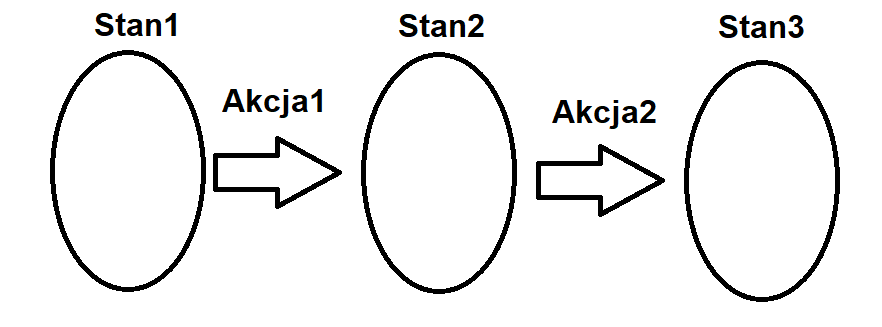
\includegraphics[scale=0.5]{PlanningGraph}
        \centering
        \caption{Najogólniejsza forma grafu planującego. Składa się on z węzłów, zwanych stanami oraz krawędzi zwanych akcjami. Docelowo poszczególne 
        stany oraz akcje są parami różne, jednak mogą zajść sytuacje, gdy powtórzenie któregoś z komponentów będzie wymagane do uzyskania odpowiedniego
        celu.}
        \label{PlanningGraph}
    \end{figure}
    Pierwotną ideę grafu planującego przedstawiono na obrazku \ref{PlanningGraph}. W trakcie dalszego omawiania metodologii GRAPHPLAN powyższa 
    rycina będzie pojawiała się ponownie z coraz to większym poziomiem szczegółowości.
    Ze względu na fakt, iż Graphplan opiera się na języku STRIPS musi mieć jasno zdefiniowane: stan początkowy, akcje oraz cel, który pragniemy uzyskać.
    Dzięki swojej strukturze Graphplan w swojej naturze podobny jest do programowania dynamicznego.

\section{Warunki początkowe}
    \label{RozdzialWarunkiPoczatkowe}
    \begin{definition}
        \label{ZasadaSwiata}
        \textbf{Zasada zamkniętego świata} - Zasada, wedle której pojęcia, które nie są ściśle opisane w świecie są nieprawdziwe.
    \end{definition}
    GRAPHPLAN, w odróżnieniu od człowieka, musi być w posiadaniu całej wiedzy o świecie, aby móc rozpocząć działanie. Przez całą wiedzę o świecie rozumie się
    posiadanie informacji na temat każdego obiektu oraz jego stanu. Wiąże się to ściśle z faktem,
    iż GRAPHPLAN operuje zgodnie z definicją \ref{ZasadaSwiata}. 
    Przed dalszą częścią pracy należy dokonać pewnego wyróżnienia. Słowo \textbf{stan} pojawia się w dwóch znaczeniach:
    stan jako pojedyncza informacja o obiekcie w świecie (Przykład: klocek B na stole numer 3) oraz stan, jako zbiór wszystkich takich informacji w danym momencie czasu.
    Z tego względu wprowadzono nowe pojęcie- "Poziom stanów", które należy stosować jako oznaczenie wszystkich informacji o świecie w danym momencie.
    \begin{definition}
        \label{PoziomStanow}
        \textbf{Poziom stanów} - Zbiór informacji o stanach wszystkich obiektów w świecie w danej jednostce czasu \textit{t}
    \end{definition}
    Szczególnym poziomem stanów jest poziom oznaczany jako pierwszy i nazywany \textbf{Warunkami początkowymi}, którego poprawne zdefiniowanie jest kluczowym aspektem w kontekscie
    uzyskania poprawnego wyniku przez algorytm.
    Analizując ponownie przykład \ref{Przyklad1} mylnym jest myśleć, iż jedyną informacją, jaką algorytm powinien posiadać o świecie jest pobyt klocka A na lewej platformie. Również
    istotną informacją jest brak klocka na platformie prawej, czyli informacja, ze jest on \textit{pusty}. Mimo poczucia nadmiarowości tej informacji, w dalszej części pracy wyjaśni
    się, dlaczego ta informacja jest niezbędna do uzyskania poprawnego wyniku.
    Przykład świata przedstawionego oraz skonstruowanego dla niego stanu początkowego:
    \begin{figure}[H]
        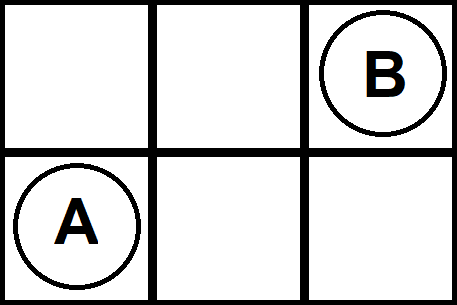
\includegraphics[scale=0.5]{PrzykladSP}
        \centering
        \caption{Przykładowy moment startowy przyszłego planu. Za pomocą okręgów oznaczono roboty, natomiast poprzez kwadraty oznaczone są kafelki- miejsca,
        po których mogą poruszać się roboty.}
        \label{PrzykladSP}
    \end{figure}
    Na powyższym przkładzie, zgodnie z ideą Graphplanu wyszczególniamy 6 stanów początkowych. Dodatkowo należy doprecyzować pojęcie bycia robota na danym kafelku. Wykonano to 
    przy pomocy dwuargumentowej relacji \textit{na}, która jako pierwszy argument przyjmuje sygnaturę robota, a na drugim- numer kafelka. Na potrzeby przykładu ustalono, iż 
    numerowanie odbywa się rzędami od lewej do prawej. Zgodnie z tymi ustaleniami pozycję robotów A i B możemy określić w następujący sposób: \textit{$na(A,4)$} oraz 
    \textit{$na(B,3)$}. Również pustość kafelków należy sformalizować wprowadzając relację jednoargumentową o nazwie \textit{pusty}, która przyjmuje jako argument numer
    pustego kafelka. Reasumując, zbiorem stanów początkowy dla analizowanego przykładu \ref{PrzykladSP} jest: 
    \begin{equation}
        \{pusty(1),pusty(2),na(B,3),na(A,4),pusty(5),pusty(6)\}
        \label{ZbiorPoczatkowy}
    \end{equation}
\section{Akcje}
    \label{RozdzialAkcje}
    Posiadając dobrze określony stan początkowy następnym krokiem będzie zdefiniowanie akcji. Zgodnie z \ref{Akcje} oraz wzmiance o akcjach w planerze STRIPS,
    akcja musi składać się z trzech komponentów:
    \begin{itemize}
        \item Czynności
        \item Warunków zajścia
        \item Efektów zajścia
    \end{itemize}
    Z tego powodu każdą z akcji będziemy traktować jako trójkę 
    \begin{equation}
        A=(C,W,E)
    \end{equation}
    gdzie każda z liter odpowiada pierwszej literze wyżej wymienionego pojęcia. 
    W skład efektów wchodzą dwa pojęcia wprost z terminologii STRIPS- dodające i usuwające. Dzięki takiemu podziałowi łatwiejszym będzie 
    zachowanie silnego podziału między przyczynami a efektami akcji. 
    Jedyną czynnością, którą należy brać pod uwagę w ramach \ref{PrzykladSP} jest czynność \textit{ruch}, którą definiujemy jako trzyargumentową relację:
    \begin{equation}
        ruch(R,S,D)
    \end{equation}
    , gdzie R odpowiada robotowi, który musi się przemieścić z kafelka oznaczonego literą S (kafelek startowy) na kafelek oznaczony
    literą D (kafelek docelowy).
    
    Następnymi składowymi są odpowiednio \textit{Warunki} jak i \textit{Efekty}. Warunki traktujemy jako zbiór wszystkich stanów, które muszą być 
    prawdziwe w danej jednostce czasu. Jeśli choć jeden stan nie jest spełnialny, opisywana akcja nie może zostać wykonana w danym ruchu.
    Efekty natomiast definiujemy jako następującą parę:
    \begin{equation}
        E=(D,U)
    \end{equation}
    gdzie D oznacza efekty dodające, a U- efekty usuwające.
    \begin{figure}[H]
        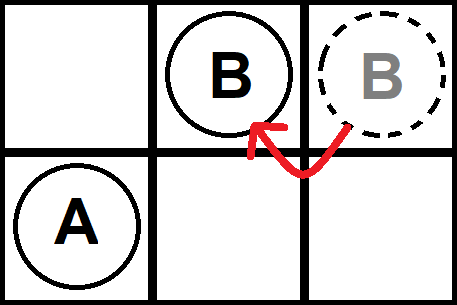
\includegraphics[scale=0.5]{PrzykladRuch}
        \centering
        \caption{Obrazowe przedstawienie ruchu robota B z kafelka 3 na kafelek 2}
        \label{PrzykladRuch}
    \end{figure}
    Niech rozpatrywaną akcją będzie przemieszczenie robota B z pozycji 3 na pozycję 2,
    przedstawiona na \ref{PrzykladRuch}. Biorąc pod uwagę, iż stanem początkowym jest \ref{ZbiorPoczatkowy} Warunkami zajścia zdarzenia
    będą: $na(R,S)$ oraz $pusty(D)$. Dla efektów natomiast sytuacja wygląda następująco: efektami dodającymi są $na(R,D)$ oraz $pusty(S)$, które informują o tym, iż klocek 
    wykonał ruch z kafelka S na kafelek D, a efektami usuwającymi $\sim na(R,S)$ oraz $\sim pusty(D)$, które informują o tym, iż kafelek S został zwolniony, 
    oraz robot nie znajduje się już na kafelku S. Przy pomocy matematycznego symbolu negacji wyrażono nieprawdziwość danego stanu. Ze względów estetycznych 
    oraz ułatwiających analizowanie pracy negacje stanów w dalszej części pracy wyrażono również przy pomocy polskiej partykuły przeczącej \textbf{nie}. 
    Dla przykładu pojęcia $\sim pusty(1)$ oraz $niepusty(1)$ z perpsektywy wprowadzonej terminologii są tożsame. 

        Posiadająć następującą wiedzę poniżej zdefiniowano jedyną akcję znajdująca się w prezentowanym przykładzie:
    \begin{equation}
        \label{Ruch}
        A=(ruch(R,S,D),\{na(R,S),pusty(D)\},\{na(R,D),pusty(S),\sim na(R,S),\sim pusty(D)\})
    \end{equation}
    Podstawiając za $R=B$, $S=3$, a $D=2$ otrzymujemy następującą akcję:
    \begin{equation}
        A=(ruch(B,3,2),\{na(B,3),pusty(2)\},\{na(B,2),pusty(3),\sim na(B,3),\sim pusty(2)\})
    \end{equation}
    
    Analogicznie można zdefiniować ruch na kafelek numer 6, oraz dwa ruchy dla robota o sygnaturze A.


    \subsection{Typy akcji}
    Definicja \ref{ZasadaSwiata} znajduje również swoje odzwierciedlenie w akcjach. Niech rozpatrywanym przykładem będzie wciąż przykład \ref{PrzykladSP}.
    W pierwszym kroku wykonano akcję $ruch(B,3,2)$.Z persepktywy człowieka jest to wystarczająca informacja, aby móc wydedukować, co we wskazanym etapie
    generowania planu  dzieje się z robotem \textbf{A}. Otóż robot A w pierwszym ruchu zostaje na tym samym kafelku. 
    Jednakże ze względu na zamkniętość świata 
    algorytmu należy go również poinformować go o tym, w jakim stanie po pierwszym kroku ma znajdować się robot A. Wykonywane jest to przy pomocy 
    akcji, zwanych \textbf{akcjami potrzymującymi}.
    \begin{definition}
        \label{Persist}
        \textbf{Akcja podtrzymująca} - Akcja, która przenosi stan obiektu w czasie $t$ nienaruszonym do poziomu stanów w czasie $t+1$
    \end{definition}
    Akcjami podtrzymującymi należy również informować świat o stanach kafelków, które nie brały udziału w akcji robota B. Przykładem takiego jest 
    kafelek 1, który w stanie początkowym, jak i w stanie następnym ciągle zachowuje swój stan jako pusty. Akcje podtrzymujące oznaczono 
    słowem kluczowym \textbf{zostań}
    Ponadto akcja typu \textit{ruch}, które aktywnie zmienia stan świata w dalszej części pracy otrzyma miano \textbf{akcji aktywnej}.
    \begin{definition}
        \label{Active}
        \textbf{Akcja aktywa} - Akcja, która zmienia stan obiektu między stanami w czasie $t$ i $t+1$.
    \end{definition}

    Posiadając powyższy podział akcji poniżej przedstawiono pełen zbiór akcji w pierwszym kroku algorytmu. Wartym odnotowania jest, iż ze względów
    estetycznych podawawnie akcji podtrzymujących będzie często pomijane, jednakże nie można zapomnieć o ich występowaniu oraz o ich kluczowej roli 
    w generowaniu precyzyjnego planu.
    \begin{align*}
        Akcje &= \{zostan(pusty(1)),zostan(pusty(2)),zostan(pusty(5)),zostan(pusty(6)),zostan(na(B,3)), \\
        &zostan(na(A,4)),ruch(B,3,2),ruch(B,3,6),
        ruch(A,4,1),ruch(A,4,5)\}
    \end{align*}
    Należy również nadmienić, iż podobnie jak w stanach, dla akcji wprowadza się pojęcie \textbf{Stanu akcji}, które funkcjonuje jako zbiór 
    składający się ze wszystkich możliwych akcji do wykonania w danej jednostce czasu.
    \begin{figure}[H]
        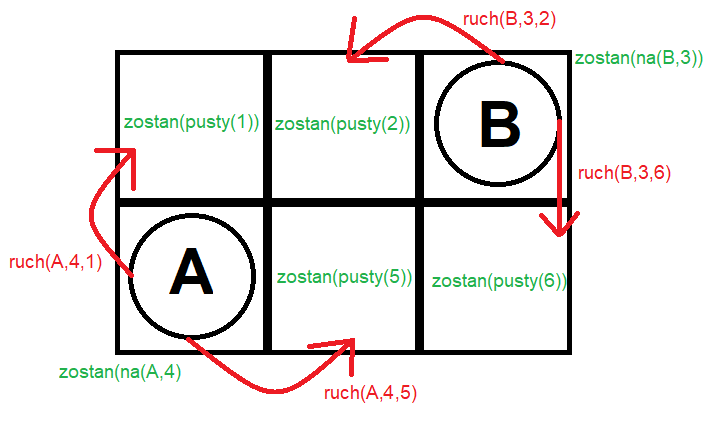
\includegraphics[scale=0.5]{PrzykladAkcje}
        \centering
        \caption{Obrazowe przedstawienie wszystkich akcji w pierwszym kroku algorytmu, akcje opisane przy użyciu czcionki o kolorze zielonym 
        symbolizują akcje podtrzymujące, natomiast o kolorze czerwonym- akcje aktywne}
        \label{PrzykladAkcje}
    \end{figure}
    

\section{Definiowanie świata}
    Zdecydowanie najtrudniejszym aspektem modelowania świata jest dokładne przedstawienie wszystkich zależności, jakie algorytm musi znać,
    aby mógł bezbłędnie wnioskować w prezentowanej przestrzeni. Analizując przykład \ref{PrzykladSP} dokonano przedstawienia schematu 
    generowania poziomu stanów początkowych oraz poziomu akcji. Zadając pytanie algorytmowi \textit{Jakie działania należy podjąć, aby jak najszybciej
    przesunąć robota A z klocka 4 na klocek 6} algorytm odpowie w następujący sposób: $ruch(A,4,6)$, jednakże przyglądając się uważnie przedstawionemu światu 
    zauważono, iż taki plan byłby realny jedynie, gdyby akcja $ruch$ oznaczała latanie- wtedy faktem jest, iż istnieje możliwość pominięcia kafelka 5 podczas 
    przemieszczenia. Niespójnośc ta pojawiła się z faktu, iż w żadnym momencie nie określono w jaki sposób dokładnie funkcjonuje czynnośc oznaczona jako \textit{ruch}.
    Wedle definicji \ref{Ruch} wszystkie warunki, aby robot mógł przemieścić się z kafelka 4 na 6 zostały spełnione.

    Naprawić ten problem można przy pomocy uściślenia wykonywanej czynności. Do tego potrzebne będzie wprowadzenie relacji \textit{sąsiad}, która 
    przyjmuje dwa argumenty- numery kafelków, które ze sobą sąsiadują. Zakładając, iż sąsiadujące kafelki to takie, które mają wspólną ścianę, sąsiadami 
    kafelka 1 są kafelki: 2 oraz 4. Dla pozostałych przestrzeni dokonano analogicznego wygenerowania listy sąsiadów. Dzięki tej operacji, 
    akcję ruch zdefiniowano w następujący sposób:
    \begin{equation}
        ruch(R,S,D) \textnormal{:-} sasiad(S,D)
    \end{equation}
    Czynność ruchu w powyższym przypadku została określona zgodnie z semantyką języka programowania \textbf{PROLOG}. Należy to rozumieć w następujący sposób:
    po lewej stronie znaku \textbf{:-} znajduje się \textit{konkluzja}, natomiast po prawej- \textit{przesłanka}. Naturalnym odczytem przedstawionej sytuacji
    będzie zdanie \textit{"Jeśli kafelki S i D są sąsiadami to możliwym do wykonania jest ruch między tymi kafelkami"}
    \begin{figure}[H]
        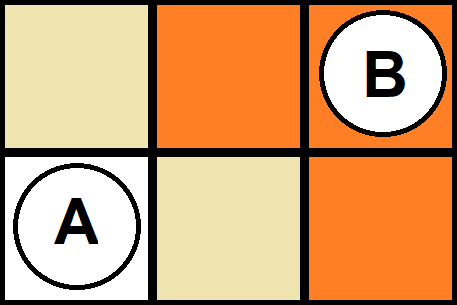
\includegraphics[scale=0.5]{PrzykladSasiad}
        \centering
        \caption{Graficzne przedstawienie relacji sąsiedztwa dla kafelka numer 4. Kolorem kremowym oznaczono miejsca, z którymi sąsiaduje, natomiast 
        pomarańczowym- te, z którymi nie sąsiaduje. Oznacza to, iż do kafelków pomarańczowych nie można dostać się wykonując jeden ruch}
        \label{PrzykladAkcje}
    \end{figure}
    Taka definicja ruchu pozwala w skuteczny sposób oddać intuicję, która wynika z poglądowego obrazka przedstawiającego rozpatrywany świat.
    Niewystarczającym jest określenie relacji $sasiad(1,2)$, gdyż wedle tego faktu kafelek pierwszy sąsiaduje z kafelkiem drugim, jednakże nie oznacza 
    to, iż kafelek drugi sąsiaduje z kafelkiem pierwszym. Z tego dla każdej pary kafelków A i B do zbioru sąsiadów należy dodać dwie relacje:
    $sasiad(A,B)$ oraz $sasiad(B,A)$. Inna sytuacja byłaby, gdyby ruch był możliwy jedynie w jedną stronę, jednakże tutaj taki stan rzeczy nie występuje.


    Oprócz definicji sąsiedztwa należy również zabezpieczyć się przed sytuacją, gdy dwa roboty będą chciały w tym samym momencie znaleźć się na tym samym 
    kafelku. Dodatkowo kafelek A nie może znajdować się w dwóch stanach jednocześnie: $pusty(A)$ oraz $na(R,A)$, gdzie R oznacza dowolnego robota. 
    Wymodelowanie tych ograniczeń jest prostym, lecz istotnym zadaniem implementując przedstawianą metodologię, które zostanie poruszone w ramach 
    przedstawiania pojęcia "wzajemnego wykluczania".
    
    
    Odpowiednie wymodelowanie świata wedle wzorców języka STRIPS może wydawać się trudnym oraz żmudnym zajęciem, jednakże przebrnąwszy 
    przez ten etap algorytm jest zwarty i gotowy do generowania planów dla wprowadzonych celów.


\section{Warstwy grafu}
    Składowe planu grafującego można podzielić na dwa typy: jeden, wyszczególniony jako poziomy stanów oraz drugi- poziomy akcji. Aby lepiej 
    uwidocznić zależność poziomu akcji od warunków początkowych oraz zależność kolejnego poziomu stanów od efektów akcji graf planujący 
    z \ref{PlanningGraph} ulegnie lekkiej modyfikacji. 
    \begin{figure}[H]
        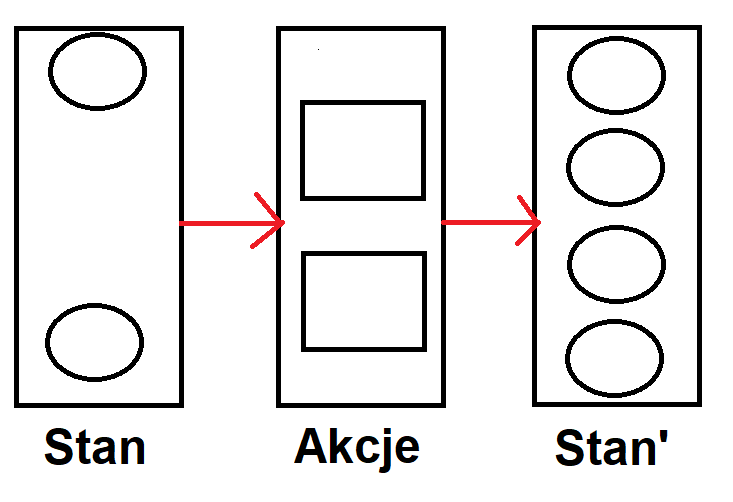
\includegraphics[scale=0.5]{PlanningGraphStates}
        \centering
        \caption{Modyfikacja do grafu planującego wprowadzona w poprzednich podrozdziałach. Wprowadzono zależności akcji od stanu poprzedniego, oraz stanu 
        następnego od akcji.}
        \label{PlanningGraphStates}
    \end{figure}
    Następnym krokiem będzie wprowadzenie definicji \textbf{Warstwy grafu}
    \begin{definition}
        \label{Warstwa}
        \textbf{Warstwą} - grafu nazywamy połączenie poziomu stanów oraz wynikającego z niego poziomu akcji
    \end{definition}
    Przez $i$-tą warstwę grafu oznaczono stan świata w $i$-tym momencie czasu. Ze względu na charakterystykę planera czas traktowany jest w sposób dyskretny-
    każda ze zdefiniowanych akcji zajmuje zawsze tyle samo czasu oraz zawsze kończy się tym samym efektem. Poziomy stanów jak i poziomy akcji 
    należące do tej samej $i$-tej warstwy nazywamy poprzez dołączenie do ich nazwy numera, odpowiadającego obecnej iteracji algorytmu
    iteracji algorytmu.
    \begin{figure}[H]
        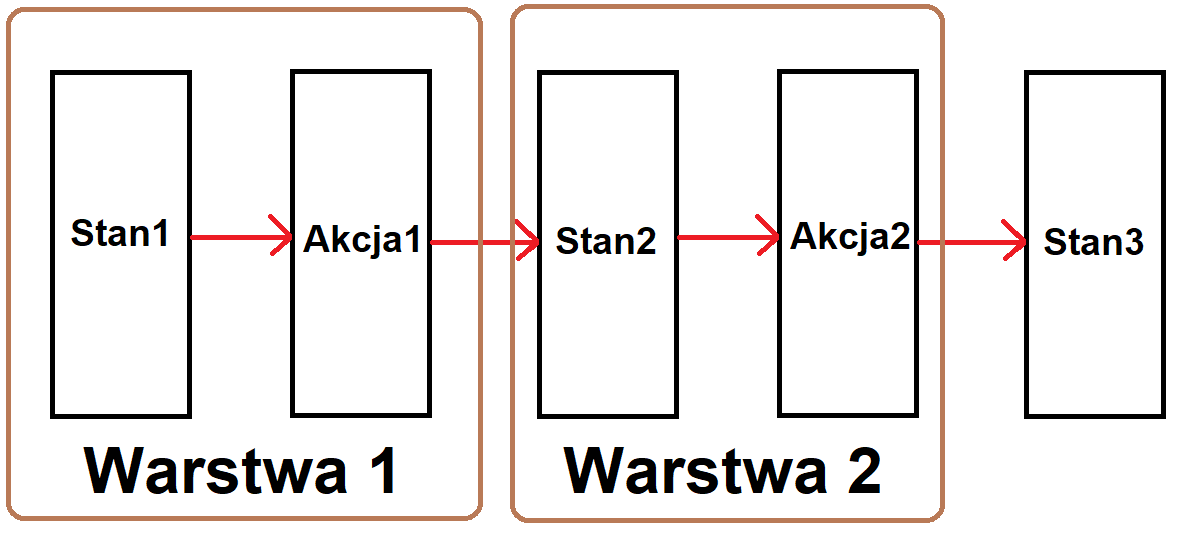
\includegraphics[scale=0.5]{PlanningGraphLevels}
        \centering
        \caption{Przedstawienie sposobu wyznaczania warstw w algorytmie planującym. Poziom stanów oraz akcji wchodzący w skład danej warstwy 
        wyróżniony jest poprzez konkatenację nazwy oraz liczby symbolizującej numer warstwy.}
        \label{PlanningGraphLevels}
    \end{figure}
    Dzięki wprowadzeniu definicji warstwy po wygenerowaniu 
    planu natychmiast wiadomo ile kroków należy wykonać, a co za tym idzie- ile czasu należy poświęcić, aby osiągnąć ustalony cel. 

    \section{Równoległość}
    \label{Rownoleglosc}
    W poprzednich paragrafach na pojedynczym poziomie akcji rozpatrywano conajwyżej jedną akcję aktywną, jednakże główną siła GRAPHPLANU, jest 
    możliwość jego reprezentacji jako częściowego porządku. To pozwala w prosty sposób wprowadzić pojęcie równoległości między akcjami. 
    \begin{definition}
        \label{Warstwa}
        Dwie (lub więcej) akcje  mogą zostać wykonane \textbf{równolegle}, gdy po ich wykonaniu w tej samej warstwie $i$, warstwa $i+1$ nie będzie 
        zawierała w sobie żadnych sprzeczności.
    \end{definition}
    Przyglądając się rysunkowi \ref{PrzykladSP} od razu należy zauważyć, iż w stanie początkowym ruch robota A nie wpływa w żaden sposób na otoczenie
    robota B. Z tego względu dwie przykładowe akcje $ruch(A,4,5)$ oraz $ruch(B,3,2)$ wręcz należy wykonać w tej samej jednostce czasu, czyli w pierwszym
    poziomie akcji. 
    \begin{figure}[H]
        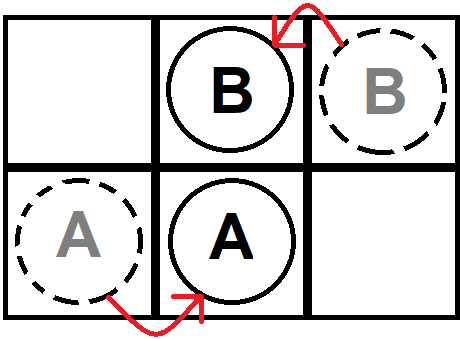
\includegraphics[scale=0.5]{PrzykladRownolegle}
        \centering
        \caption{Przykład możliwości zastosowania równoległości w planowaniu działania. Należy zauważyć, iż ruchy robotów w żaden sposób ze sobą
        nie kolidują.}
        \label{PrzykladRownolegle}
    \end{figure}
    
    Po wprowadzeniu definicji równoległości, również definicja kroku musi ulec ewolucji. 
    \begin{definition}
        \label{Krok}
        \textbf{Krokiem} algorytmu nazywamy zbiór wszystkich możliwych do realizacji akcji w danej warstwie.
    \end{definition}
    Dzięki naniesionej poprawce pozbywamy się łatki mówiącej o tym, iż pojedyncza zmiana stanu jest ściśle związana z jedną akcją.W tym miejscu należy 
    zauważyć, iż poprzednie analizy zawierały spore uproszczenie, gdyż akcje podtrzymujące również należą do kroku algorytmu, co zostało zaprezentowane
    w trakcie kreowania pierwszej warstwy akcji dla rozpatrywanego przykładu. 

    Istnieją przypadki, gdy podmiot realizujący plan nie jest w stanie wykorzystać benefitów płynących z możliwości dokonywania akcji równolegle, 
    na przykład ze względu na ograniczone zasoby. GRAPHPLAN również rozwiązuje ten problem, pozwalając przekształcać swój częsciowy porządek 
    na porządek liniowy w dość dowolny sposób. Otóż akcje z danej warstwy mogą być wykonywane w dowolnej kolejności, gdyż w żaden sposób ze sobą nie 
    kolidują. Z persepktywy algorytmu najważniejszym jest, aby stan świata $i$ i $i+1$ był zgodny z informacjami jakie posiada o świecie. Zgodnie z
    przykładem \ref{PrzykladRownolegle} widać, iż to, czy akcja $ruch(A,4,5)$ zostanie wykonana przed akcją $ruch(B,3,2)$ lub to, czy akcja 
    $ruch(B,3,2)$ odbędzie się prxed $ruch(A,4,5)$- efekt końcowy jest identyczny.

    \subsection{Wzajemne wykluczanie}
    Twórcy algorytmy wprowadzając równoleglość, zdawali sobie sprawę z mocy tego podejścia. Dzięki temu ogromna liczba planów ulega redukcji
    jeśli chodzi o wymagany czas wykonania. Jednakże równoległość wprowadza kolejny istotny problem w prezentowanym świecie, a mianowicie- co, gdy
    wykonanie dwóch akcji będzie wprowadzało sprzeczność w następnym poziomie świata? Sytuacja ta została przedstawiona na poniższym rysunku
    \begin{figure}[H]
        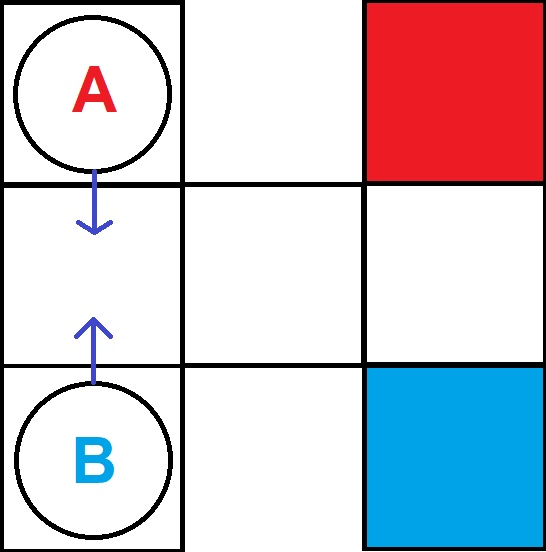
\includegraphics[scale=0.5]{PrzykladRownolegleZle}
        \centering
        \caption{Przykład świata, w którym wprowadzenie równoległości dla pierwszej warstwy algorytmu jest niemożliwe. 
        Dwa roboty próbują przejść na ten sam kafelek
        w tej samej jednostce czasu, co z perspektywy kafelka powoduje konflikt. Odpowiednio kolorami:
        czerwnoym i niebieskim oznaczono roboty, oraz kafelki, które są ich celem.}
        \label{PrzykladRownolegle}
    \end{figure}
    
    Zmusiło to twórców algorytmu do wporwadzenia pojęcia \textbf{relacji wykluczania}. 
    O akcjach wzajemnie się wykluczających (ang. actions mutually exclusive, \textbf{mutex}) wspomiano w ramach definiowana świata. Pojęcie ów można 
    określić w następujący sposób:
    \begin{definition}
        \label{Warstwa}
        \textbf{Relacją wzajemnie wykluczającą się} - jest relacją między akcjami(stanami), która informuje o tym, iż nie istnieje plan taki,
        aby dwie wybrane akcje(stany) mogły być prawdziwe w tej samej jednostce czasu $t$
    \end{definition}
    Przykładem stanów wykluczających jest para: $pusty(1)$ oraz $\sim pusty(1)$. Kafelek nie może być pusty jak i niepusty jednocześnie.
    Przykład dwóch akcji wykluczających przedstawiono na rysunku \ref{PrzykladRownolegle}. Należy zauważyć, iż wzajemne wykluczanie się 
    jest rozpatrywane warstwowo.
    Kolejnym naturalnym krokiem jest ustalenie, kiedy akcje oraz stany są ze sobą w relacji wykluczającej. 

    \subsubsection{Wykluczanie się stanów}
    Dwa stany są ze sobą w relacji wzajemnie wykluczającej w dwóch następujacych przypadkach:
    \begin{enumerate}
        \item Negacja- przypadek, w którym jeden ze stanów jest negacją drugiego
        \item Niespójne powstanie- wszystkie akcje z poprzedniej warstwy, które prowadza 
        do utworzenia ów stanów są ze sobą parami w relacji wykluczającej
    \end{enumerate}
    Ze względu na naturalność pojęcia negacji zbędnym jest wprowadzenie większego przykładu niż przedstawienie, iż dla każdego obiektu istnieje 
    para stanów znajdujących się w relacji wykluczającej. Niech za przykład posłuży pustość kafelka. Kafelek nie może być jednocześnie pusty, jak 
    i niepusty, co sprowadza się, iż stan $pusty(kafelek)$ jak i $\sim pusty(kafelek)$ są niemożliwe do zawarcia w jednej warstwie planu.

    Dla kontrastu przedstawienie przypadku, w którym zachodzi \textbf{niespójne powstawanie} jest trudniejsze i wymaga użycia 
    przykładowej ilustracji:

    \begin{figure}[H]
        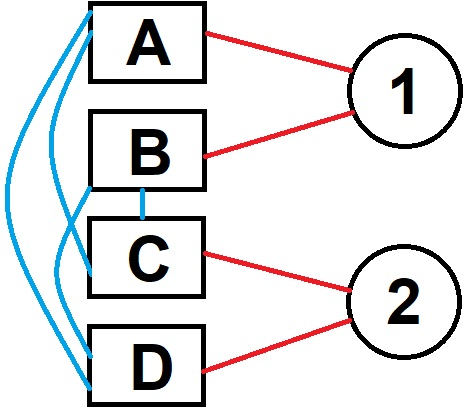
\includegraphics[scale=0.5]{PrzykladWykluczenie3}
        \centering
        \caption{Urywek planu przedstawiający sytuację, w której dwa stany powstają w sposób niespójny. Zgodnie z założeniami akcje oznaczone są przy 
        pomocy prostokątów, stany- okręgów, miedzy akcjami a stanami czerwone linie symbolizują które stany są efektami których akcji, natomiast linie
        niebieskie między akcjami symbolizują powstałe między nimi \textit{mutexy}}
        \label{PrzykladWykluczenie3}
    \end{figure}

    Zgodnie z nienaturalnym przykładem \ref{PrzykladWykluczenie3} należy zauważyć, iż stany 1 oraz 2 nie mogą 
    znajdować się jednocześnie w planie ze względu na to, iż każda z akcji, która generuje stan 1 (B,C) znajduje się w relacji 
    wzajemnie wykluczającej z każdą akcją, która generuje stan 2 (C,D). Oznacza to, iż ów dwa stany powstają w sposób \textbf{niespójny}.
    
    Z reguły ten typ wykluczeń występuje po większej liczbie kroków dla bardziej rozbudowanych światów jak i planów.
    

    \subsubsection{Wykluczanie się akcji}
    Dwie akcje mogą być ze sobą w relacji wzajemnie wykluczającej w trzech następujących przypadkach:
    \begin{enumerate}
        \item Niespójny efekt- przypadek, w którym zbiór efektów jednej z akcji 
        jest negowany przez zbiór efektu drugiej
        \item Przeszkadzanie - przypadek, w którym jedna z akcji usuwa warunki 
        zajścia akcji drugiej 
        \item Konkurencyjne potrzeby- przypadek, w którym warunki zajścia akcji 
        są ze sobą w relacji wykluczającej.
    \end{enumerate}
    Poniższe przykłady w obrazowy sposób przedstawiają każdy w wyżej wymienionych
    przypadków:

    \begin{figure}[H]
        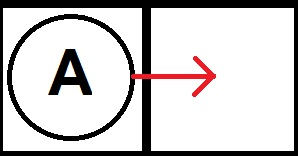
\includegraphics[scale=0.5]{PrzykladWykluczenie2}
        \centering
        \caption{Przykład wykluczania się akcji aktywnych z podtrzymującymi}
        \label{PrzykladWykluczenie2}
    \end{figure}

    Na pierwszy rzut oka wydawać by się mogło, iż niemożliwym jest wygenerowanie dwóch akcji znajdujących się w relacji wykluczania dla przykładu 
    \ref{PrzykladWykluczenie2}, jednakże istnieją dwie takie pary: 
    \begin{equation}
        zostan(na(A,lewy)),ruch(A,lewy,prawy)
    \end{equation} 
    oraz 
    \begin{equation}
        zostan(pusty(prawy)) oraz ruch(A,lewy,prawy)
    \end{equation} 
    Wynika to z faktu, iż zbiór efektów jednej akcji z powyższych par jest negowany przez drugi. Zbiorem efektów akcji 
    $zostan(na(A,lewy))$ jest $na(A,lewy)$, jednakże zbiorem efektów $ruch(A,lewy,prawy)$ jest ciut większy zbiór:
    \begin{equation}
        na(A,prawy), \sim na(A,lewy), pusty(lewy), \sim pusty(prawy)
    \end{equation}
    Widać, iż efekt $\sim na(A,lewy)$ jest negacją efektu $na(A,lewy)$. Akcje podtrzymujące i aktywne względem tego samego obiektu zawsze sobą ze sobą 
    w relacji wykluczającej ze względu na \textbf{niespójny efekt}.

    \begin{figure}[H]
        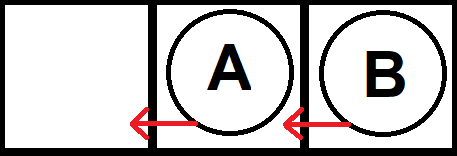
\includegraphics[scale=0.5]{PrzykladWykluczenie1}
        \centering
        \caption{Przykład świata, w którym każdy z robotów próbuje przesunąć się na sąsiadujący z lewej strony klocek. Uwidoczniona sytuacja 
        jest przykładem wykluczających się akcji}
        \label{PrzykladWykluczenie1}
    \end{figure}

    Idea przedstawiona na rysunku \ref{PrzykladWykluczenie1} jest ciekawym przykładem, pozwalającym zrozumieć dokładniej definicję słowa 
    \textbf{równoległość} odnośnie planów generowanych przez GRAPHPLAN. Gdyby roboty poruszając się z tą samą szybkością ruszyły w tym samym momencie
    to wykonanie ów sekwencji akcji byłoby w zupełności możliwe, jednakże w sekcji \ref{Rownoleglosc} wspomniano, iż każdy z wygenerowanych planów 
    musi być możliwy do przedstawienia w postaci porządku liniowego, czyli plan równoległy może zostać przerobiony w dowolny sposób na plan,
    w którym każda z akcji wykonywana jest po kolei. Zgodnie z omawianym przykładem sprowadzenie ów planu do dowolnej postaci liniowej jest 
    niemożliwe, gdyż istnieje konfiguracja, w której to najpierw robot B miałby wykonać ruch, jednakże jest to niemożliwe ze względu na 
    obecność robota A na kafelku będącym jego celem podróży. Dodatkowe wprowadzenie ograniczeń na konwersję planów równoległych na liniowe 
    jest bardziej skompilowanym zagadnieniem, którego omówienie nastąpi w sekcji odpowiedzialnej za możliwe rozwinięcia algorytmu.
    
    Z powyższego opisu wynika, iż 
    omawiane relacje ruchu są ze sobą w relacji wzajmenie wykluczającej z powodu \textbf{przeszkadzania}. 
    Klocek A do wykonanaia ruchu potrzebuje znajdować się na kafelku środkowym, co oznacza, iż kafelek środowy musi byc niepusty, 
    jednakże klocek B potrzebuje, aby ów klocek był pusty. Relacja wykluczająca między tymi stanami bezpośrednio generuje wykluczanie się tych akcji.
    
    Ponadto, omawiane akcje w ilustracji \ref{PrzykladWykluczenie1} znajdują się w relacji wykluczającej z powodu \textbf{Konkurencyjnych potrzeb}. 
    Robot B przy przesunięciu \textbf{na} środkowy kafelek wymaga, aby on był pusty, natomiast robot A przy przesunięciu \textbf{z} środkowego klocka 
    musi się na nim znajdować, czyli kafelek musi być niepusty. Stany pusty i niepusty względem kafelka są w oczywistej relacji wykluczającej 
    co automatycznie generuje wykluczenie się wspomnianej pary akcji. Przykład ów przedstawia, iż jedna para akcji może być ze sobą w relacji wykluczającej 
    z kilku powodów, jednakże algorytm rozpatrując parę akcji podchodzi do tego w sposób binarny, co oznacza, iż patrzy jedynie czy znajdują się w 
    relacji wykluczającej czy nie, nie interesuje go liczba sposobów, na które ów relację można utworzyć.    

    Należy zauważyć, iż dzięki wprowadzeniu relacji wzajemnego wykluczania pozbyto się porównań wielu akcji, których zajście jest niemożliwe w tej samej 
    warstwie grafu. Koszt jaki został poniesiony ze względu na zapamiętywanie dodatkowych informacji o relacjach między akcjami jest często zaniedbywalny,
    ze względu na ogrom benefitów w postaci mniejszej liczbie sprawdzeń, a co za tym idzie- szybsze działanie algorytmu.


\section{Wyszukiwanie planu}
    Zdefiniowawszy wszystkie niezbędne elementy planera należy wskazać, w jaki sposób przy posiadaniu całej wiedzy wygenerowanej przez graf planujący.
    Wykonywane jest to w następujący sposób:
    \begin{enumerate}
        \item Rozpoczynając od stanu początkowego, zgodnie z opisanymi w poprzednich sekcjach metodami, odbywa się generowanie kolejnych warstw grafu,
        biorąc pod uwage informację o \textbf{mutexach} między akcjami oraz stanami
        \item Dla każdej nowo utworzonej warstwy $i$ dokonywane jest sprawdzenie, czy wszystkie założenia z celu nie znajdują się 
        w ów poziomie stanów. Jeśli odpowiedź jest negatywna, odbywa się dalsze generowanie planu zgodnie z 1. Jednak, gdy 
        wszystkie stany celu znajdują się na poziomie $i$ dochodzi do generowania planu.
        \item Dla każdego stanu z celów na poziomie $i$ dochodzi do wybrania akcji, dzięki której został on wygenerowany. 
        Ów operacja dokonywana jest dla każdego stanu. Jeżeli dobrane akcje są ze sobą w relacji wykluczającej, należy spróbować innej 
        kombinacji akcji. Jeśli wszystkie dobory akcji zawiodą należy wygenerować kolejną warstwę grafu i ponownie, w warstwie $i+1$, rozpocząc cały proces
        \item Jeśli jednak istnieje dobór akcji taki, że nie występuje między nimi relacja wykluczania, należy dla każdego stanu 
        znajdującego się w zbiorze warunków zajścia wspomnianych akcji wykonać procedurę z kroku 3. 
        \item Jeśli dojdzie do niepowodzenia na którymkolwiek z etapów powrotu do stanu wyjściowego algorytm podejmuje próbuję odpowiedniego dobrania 
        akcji na ostatnio sprawdzonym poziomie. Brak niepowodzenia na ścieżke powrotu od warstwy $i$ do warunków początkowych świadczy o tym, 
        iż istnieje sekwencja akcji pozwalająca otrzymać stany zdefiniowane z celu w określonym przez stany początkowe świecie, co oznacza, 
        iż jest możliwym utworzenie odpowiedniego \textbf{planu}.
    \end{enumerate}
    Aby precyzyjnie przedstawić działanie algorytmu w następnej części programu przeprowadzono rozbudową analizę konkretnego przykładu:

    \begin{figure}[H]
        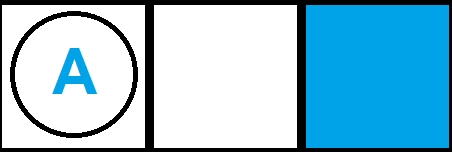
\includegraphics[scale=0.5]{PrzykladPlan1}
        \centering
        \caption{Sytuacja początkowa świata, dla którego odbędzie się przykładowe generowanie planu. Kolorem niebieskim zaznaczono kafelek docelowy robota}
        \label{PrzykladPlan1}
    \end{figure}

    \ref{PrzykladPlan1} przedstawia świat, w którym robot A z kafelka 1 próbuje przedostać się do kafelka 3 (Kafelki ponownie numerowane są od lewej strony
    do prawej).

    \begin{figure}[H]
        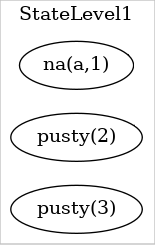
\includegraphics[scale=0.5]{PrzykladPlanStateLevel1}
        \centering
        \caption{Warunki początkowe omawianego świata. Obrazki ułatwiające analizę przykładu w całości zostały 
        wykonane przez oprogramowanie utworzone na rzecz pracy. }
        \label{PrzykladPlanWP}
    \end{figure}
    W powyższy sposób zaprezentowano stan początkowy świata. Wszystkie definicje relacji takich jak \textbf{na}, \textbf{idz}, \textbf{zostan}, czy 
    \textbf{pusty} wprowadzono w podrozdziałach \ref{RozdzialWarunkiPoczatkowe} i \ref{RozdzialAkcje}. W wygenerowanych przez oprogramowanie grafach \textbf{poziomy stanów}
    określane są poprzez swój angielski odpowiednich \textbf{StateLevel}. Podobnie z \textbf{poziom akcji} i \textbf{ActionLevel}. 

    \begin{figure}[H]
        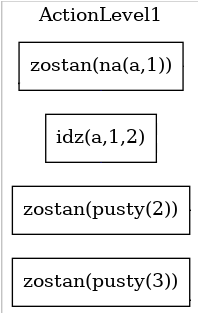
\includegraphics[scale=0.5]{PrzykladPlanActionLevel1}
        \centering
        \caption{Wygenerowane akcje na podstawie warunków początkowych}
        \label{PrzykladPlanAP1}
    \end{figure}

    Następnie przystąpiono do wygenerowania wszystkich możliwych akcji. Postąpiono zgodnie ze wskazówkami z podrozdziału \ref{RozdzialAkcje}. 
    Dodajemy niezbędne krawędzie wynikające z warunków, jak i efektów każdej z akcji oraz mutexy.

    \begin{figure}[H]
        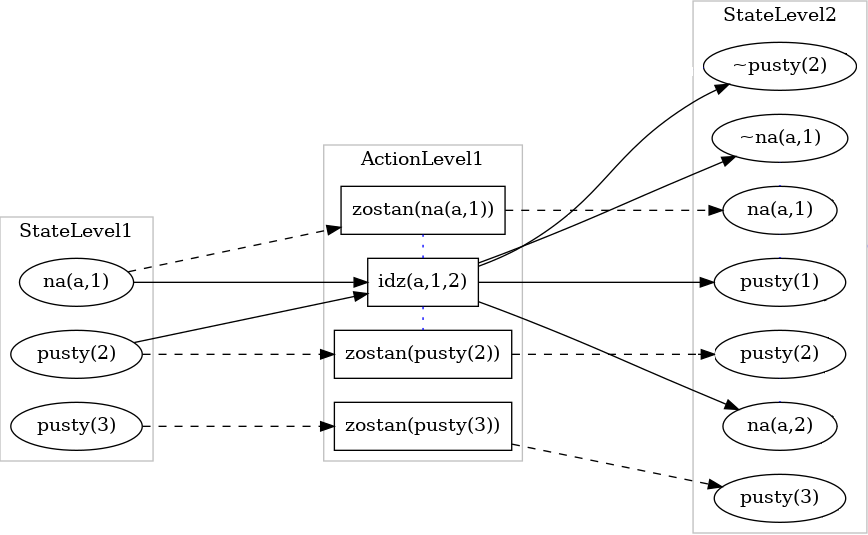
\includegraphics[scale=0.5]{PrzykladPlanWarstwa1}
        \centering
        \caption{Wygenerowany drugi stan grafu bezpośrednio wynikający z pierwszego poziomu akcji}
        \label{PrzykladPlanW1}
    \end{figure}

    Przy pomocy efektów akcji automatycznie wykreowano następny poziom stanów. Zgodnie z schematem planowania należy sprawdzić, czy oczekiwany cel
    $na(A,3)$ znajduje się w zbiorze stanów poziomu drugiego. Po szybkiej analizie okazuje się, iż cel nie znajduje się na wskazanym poziomie, więc
    należy dokonać rozszerzenia grafu planującego o kolejny poziom. Następuje to w sposób analogiczny.



\section{Własności GRAPHPLAN'u}

\section{Prosty przykład}
